\Large\textbf{}\\
\Large\textbf{Use Case 13 - Navigazione nello spazio tridimensionale} \\
\vspace{0.5cm}
\begin{figure}[h]
 \centering
 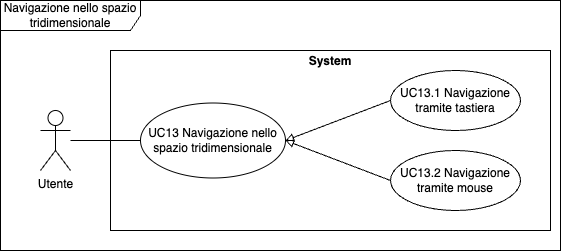
\includegraphics[width=0.8\textwidth]{UseCasesImages/Navigation.png}
\end{figure}
\large\textbf{} \\
\textbf{Attori:} User\\
\textbf{Pre-condizione:} L'utente si trova nello spazio tridimensionale\\
\textbf{Post-condizione: } L'utente ha effettuato un movimento nello spazio tridimensionale\\
\textbf{Scenario Principale:} L'utente effettua un movimento nello spazio tridimensionale attraverso l'utilizzo del mouse o della tastiera\\
\textbf{Generalizzazioni:} 
\begin{itemize}
    \item UC14 Navigazione tramite tastiera
    \item UC15 Navigazione tramite mouse
\end{itemize}
\vspace{0.5cm}